This section is a list of all possible use cases for the application. The team will use this to build on to create functional requirements which together help create a design for the application. The table below shows a description of a use case, the actors involved in it, the cause for the use case, the action needed as a result and the expected outcome. Note the following table is not ordered.\\
\begin{table}[H]
\caption{List of use cases.}
\begin{tabularx}{\linewidth}{|X|X|X|X|X|X|X|}
\hline
\multicolumn{7}{c}{ Use cases } \\
\hline
ID & Description & Actors & Pre-conditions & Main effect & Post-conditions & Category/ package \\
\hline
UC1 & Cash register. & Employees. Manager. Owner. & Customer makes an order and pays for it. & Cash is added to the cash register. & Cash is stored in the cash register and correct change is given. & Front of house/ Cheeseburger. \\
\hline
UC2 & Add item to order. & Employees. Manager. Owner. & Customer orders an item/items. & Add requested item to the current order. & Item(s) added to the current order and total price updated. & Front of house/ Cheeseburger. \\
\hline
UC3 & Remove item from order. & Employees. Manager. Owner. & Customer no longer desires a specific item/items in the current order. & Remove undesirable item from the current order. & Item(s) are removed for the current order and total price updated. & Front of house/ Cheeseburger. \\
\hline
UC4 & Cancel order. & Employees. Manager. Owner. & Customer no longer wants to order from our truck. & Remove all items from the current order. & All items removed from the current order and total price updated. & Front of house/ Cheeseburger. \\
\hline
UC5 & Refund order. & Employees. Manager. Owner. & A customer returns an item that was incorrect and or not up to standard. & Refund the total cost of the returned item. & Complaint is noted and cost of the item returned to the customer. & Front of house/ Cheeseburger. \\
\hline
UC6 & Special order. & Employees. Manager. Owner. & Customer requests a menu item be modified. & Ingredients used in creation of item changed for this case only. & Chefs are informed of special order/ ingredient change. & Front of house/ Cheeseburger. \\
\hline
UC7 & Create a menu. & Chefs. Owner. & New menu has been created and needs to be added to the system. & Add new menu to the system. & Menu is ready for use. & Management/ Boiled egg. \\
\hline
UC8 & Add a menu item. & Chefs. Owner. & Menu needs to be edited to accommodate for new item(s). & Add an item to an existing menu. & Menu is updated with new item(s). & Management/ Boiled egg. \\
\hline
UC9 & Remove a menu item. & Chefs. Owner. & Menu needs to edited to remove item(s). & Remove an item from an existing menu. & Menu is updated without removed item(s). & Management/ Boiled egg. \\
\hline
\end{tabularx}
\end{table}
\begin{tabularx}{\linewidth}{|X|X|X|X|X|X|X|}
\hline
\multicolumn{7}{c}{ Use cases } \\
\hline
ID & Description & Actors & Pre-conditions & Main effect & Post-conditions & Category/ package \\
\hline
UC10 & Edit a menu item. & Chefs. Owner. & An aspect of an existing menu item has changed. & Change details of an item on an existing menu. & Menu is updated with new information about the item. & Management/ Boiled egg. \\
\hline
UC11 & Add recipes. & Chefs. Owner. & New recipe for a given menu item is created. & Add a new recipe to the system. & Recipe is ready for use. & Management/ Onion soup. \\
\hline
UC12 & Remove recipes. & Chefs. Owner. & A specific recipe is no longer required. & Remove existing recipe from system. & Recipe is no longer available for use. & Management/ Onion soup. \\
\hline
UC13 & List recipes. & Chefs. Owner. & Recipes needed for creation of menu items. & List the recipe for a given menu item. & Recipe is open and readable so the item can be created. & Management/ Onion soup. \\
\hline
UC14 & Add ingredients (stock). & Chefs. Owner. & Order of stock has arrived. & Add new items to stock. & The new level of stock is displayed in the system. & Management/ Onion soup. \\
\hline
UC15 & Update stock. & Chefs. Owner. & Stock has been used to create menu items. & Update the stock to account for item usage. & The new level of stock is displayed in the system. & Management/ Onion soup. \\
\hline
UC16 & List available stock. & Chefs. Owner. & Chefs need to check how much of each item they can create. & View the current level of stock. & The level of stock and quantity of each menu item that can be created is displayed. & Management/ Onion soup. \\
\hline
UC17 & Check sales. & Owner. & Business hours have ended and no more sales will be made. & Check the number of sales made on a given day. & The number of sales on the given day is displayed. & Management/ Gumbo. \\
\hline
UC18 & Generate sales report. & Owner. & Owner needs a sales record to show potential investors. & Generate formal report detailing sales,costs and profits. & A report detailing sales and costs, profit margins etc is generated with visual aids. & Management/ Ginger crunch. \\
\hline
UC19 & Adjust prices. & Chefs. Owner. & The price of a given item is too high or low. & Adjust the price of a given menu item. & Menus are updated to reflect adjustment. & Management/ Onion soup. \\
\hline
UC20 & Save Menus. & Chef. Owner. & Menus changes are needed to be saved. & Menus are stored in the system. & Menus that include changes are stored. & Management/ Onion soup. \\
\hline
UC21 & Load Menus. & Employees. Manager. & Menus need to be displayed for customers to view. & Display menus. & Menus are displayed and readable. & Management/ Onion soup. \\
\hline
\end{tabularx}
\begin{table}[H]
\begin{tabularx}{\linewidth}{|X|X|X|X|X|X|X|}
\hline
\multicolumn{7}{c}{ Use cases } \\
\hline
ID & Description & Actors & Pre-conditions & Main effect & Post-conditions & Category/ package \\
\hline
UC22 & View Historical Sales. & Owner. & Owner wants to see the sales for a given day& Display sales made on the given day& The sales from the desired day are displayed. & Management/ Ginger crunch. \\
\hline
UC23 & Place Order. & Employees. Manager. & Customer has finished ordering. & Commit order to the system. & Stock levels adjusted and preparation of items begins. & Front of house/ Cheeseburger. \\
\hline
UC24 & Add Ingredients. & Chefs. Owner. & New ingredients used to create an item. & Add new ingredients to the system. & New ingredients added to the system and ready for use. & Management/ Onion soup. \\
\hline 
UC25 & Remove ingredients. & Chefs. Owner. & Ingredients no longer used to create an item. & Remove ingredients from the system. & Existing ingredients are no longer in the system. & Management/ Onion soup. \\
\hline
UC26 & Add item when stock is (critically) low. & Employees. Manager. & Customer orders an item which has critical low stock level. & Item is not able to be added to order. & Item is only added if the stock is available. & Front of house/ Cheeseburger. \\
\hline
UC27 & Check for number of servings. & Employees. Manager. & Employee is unsure of how many servings of an item can be created with given stock level. & Display an approximate number of servings left based on stock level. & Information displayed on the screen about the number of servings that can be made. & Front of house/ onion soup. \\
\hline
UC28 & Add item to production queue & Employees. Manager. & An order has been placed by the customer and needs to be prepared. & Order placed at the end of the production queue. & Order is ready to be served. & Front of house/ Cheeseburger. \\
\hline
UC29 & Remove item from production queue. & Employees. Manager. & An order has been prepared. & Order is removed from the top of the production queue. & Order is given to the customer and preparation of the next order can begin. & Front of house/ Cheeseburger \\
\hline
UC30 & Print customer order receipt. & Employees. Manager. & An order has been processed. & Order summary receipt is printed. & Receipt is given to the customer. & Front of house/ Cheeseburger. \\
\hline
UC31 & Edit recipe. & Chefs. Owner. & Change in recipe occured. & Change recipe in system. & New recipe is stored in system. & Management/ Onion soup. \\
\hline
UC32 & Delete a menu & Owner. Manager & Existing menu in the system must be removed. & Remove the existing menu in the system. & Menu is removed, without errors. & Management/ Boiled egg. \\
\hline
\end{tabularx}
\end{table}
\pagebreak
\subsection{Blue sky scenario:}
The software doesn’t break, slow down or cause the employee any confusion. This means that the food truck is able to get through customers faster and is therefore able to make sales. The analytics  also need to be correct in order for the truck is able to accommodate for all the customers as the software is rendered useless and the truck cannot make anymore sales if there is stock left to make customers orders. Therefore the speed, reliability and analytics that the software provides is very important in the success of the business.

\begin{figure}[H]
	\centering
	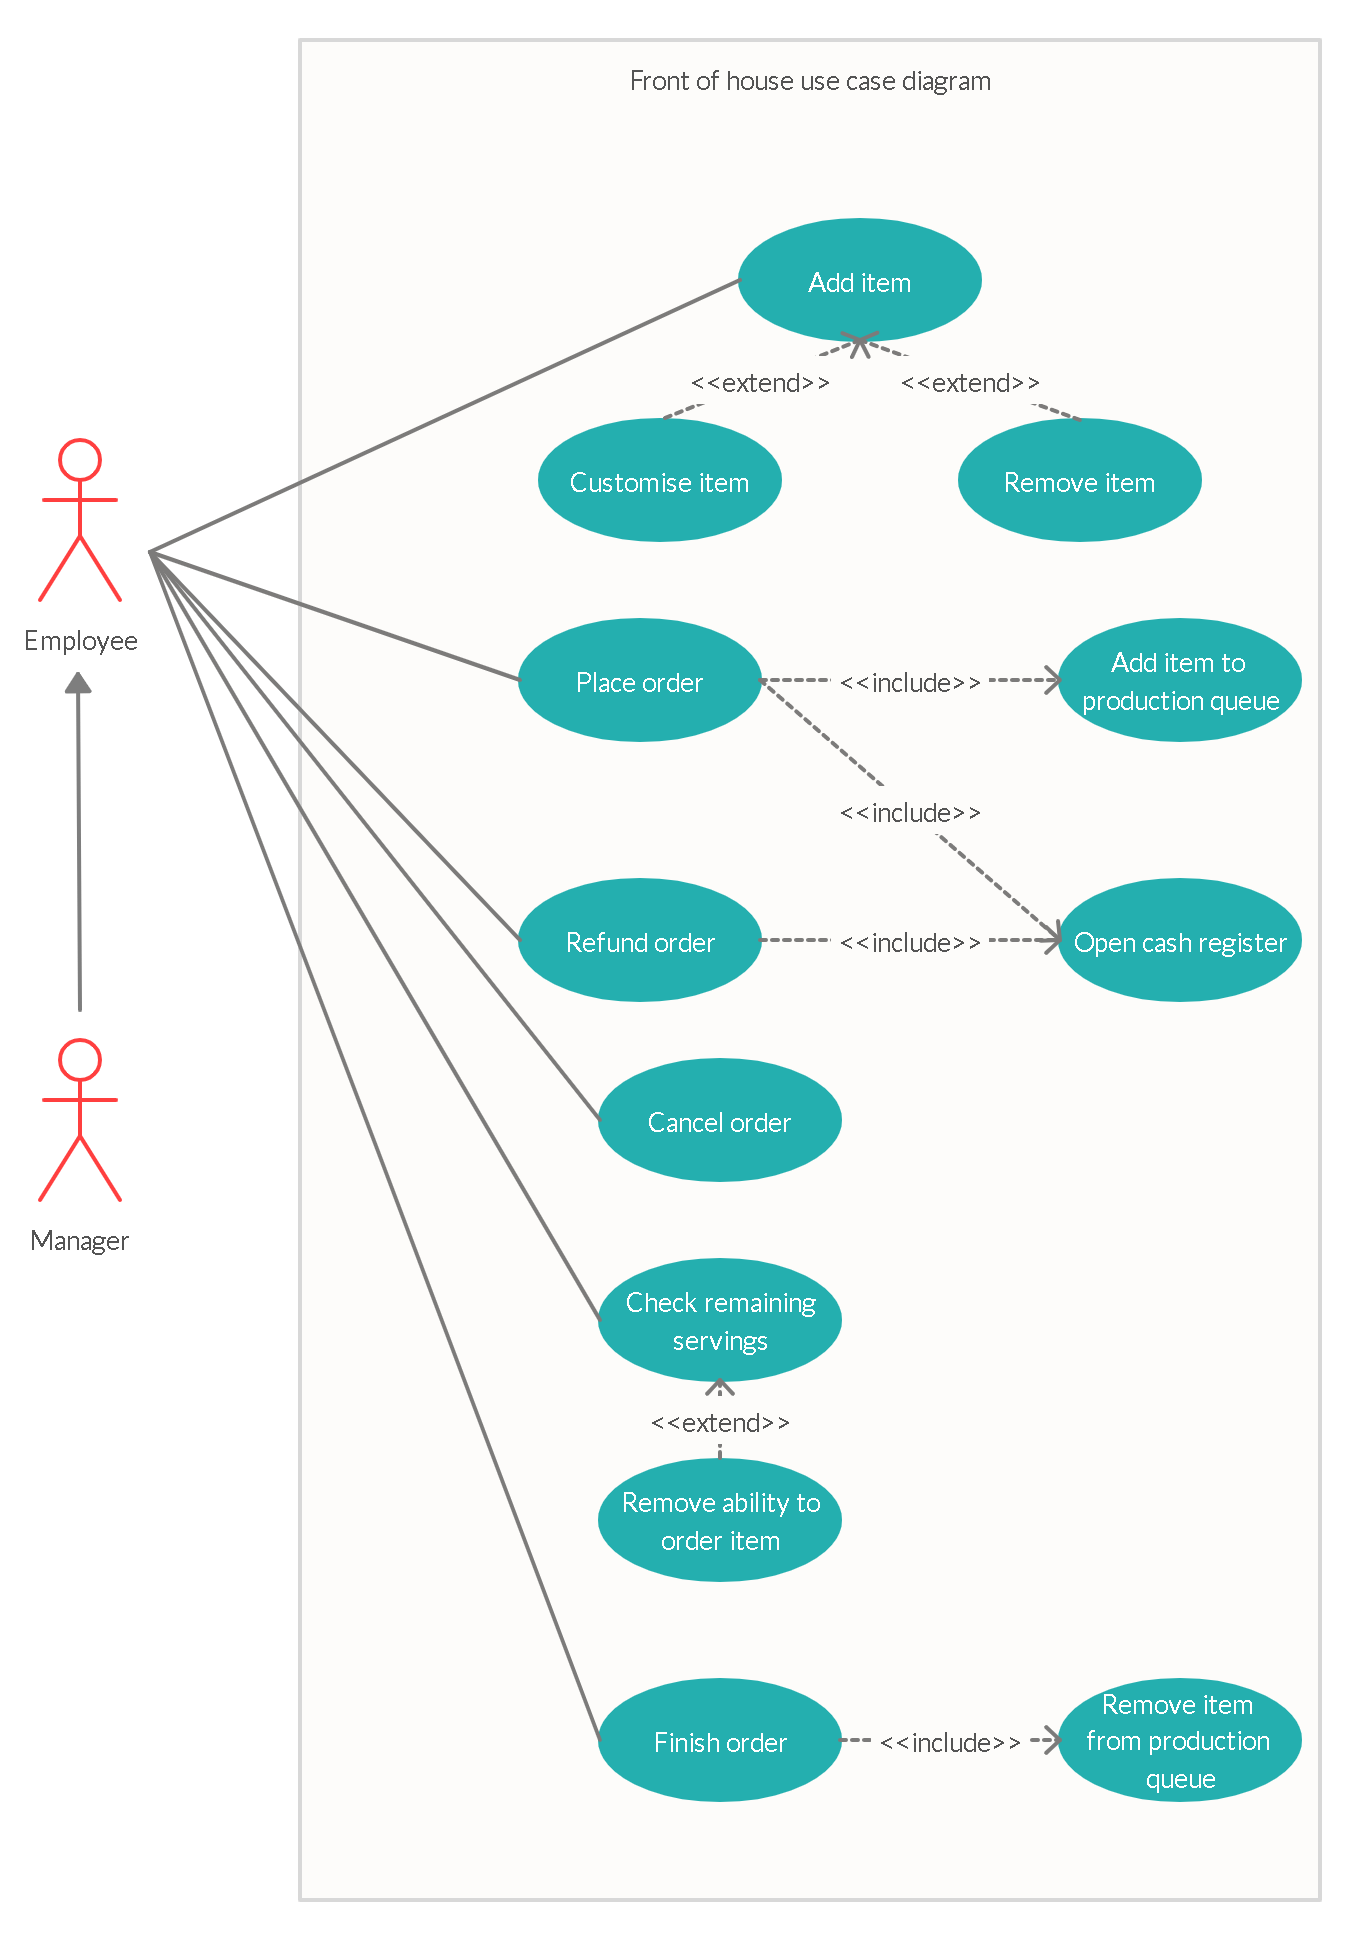
\includegraphics[width=145mm]{images/FOH_UCD.png}
	\caption{Front of house use case diagram}
\end{figure}

\begin{figure}[H]
	\centering
	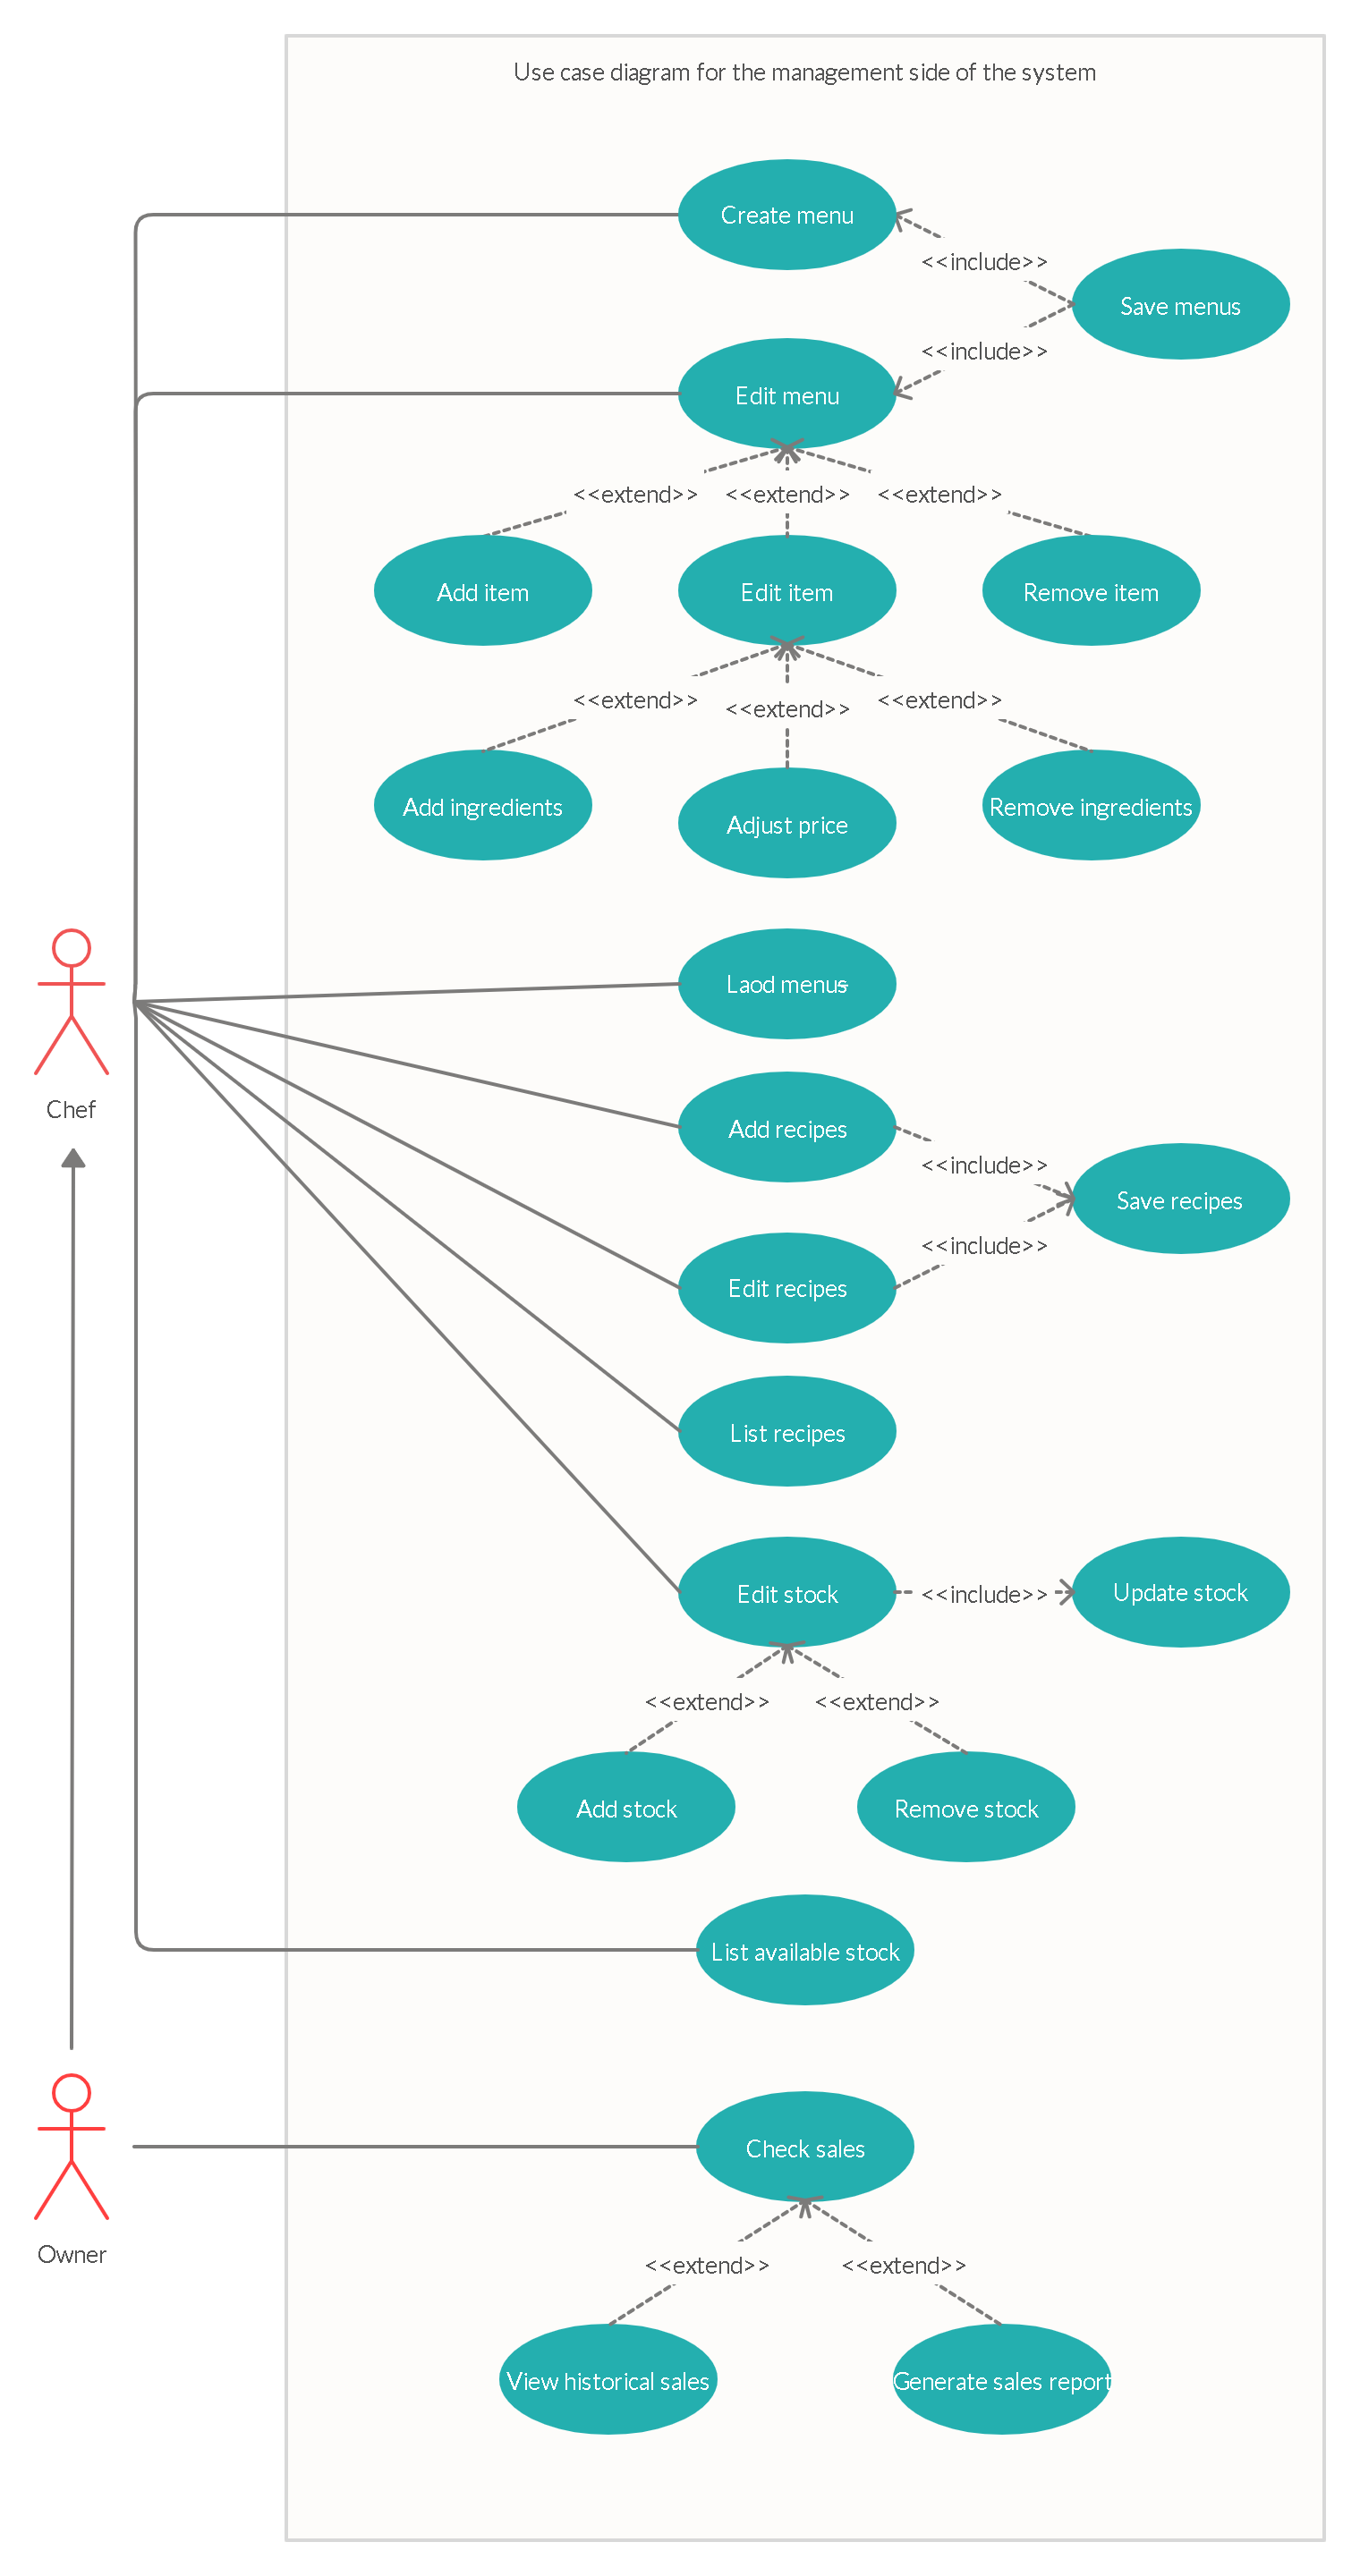
\includegraphics[width=135mm]{images/M_UCD.png}
	\caption{Use case diagram for management}
\end{figure}